\documentclass[prl,aps,epsf,showpacs,twocolumn]{revtex4}
\usepackage{times}
\usepackage{graphicx}
\usepackage{float}
\usepackage{latexsym,amsmath,amssymb,bm,euscript}
\usepackage{color}
\usepackage{subfigure}
\usepackage{epstopdf}
\usepackage[colorlinks=true,linkcolor=blue,citecolor=blue]{hyperref}
\usepackage{hyperref}

%\renewcommand{\topmargin}{0.08in}
\newcommand{\oim}[1]{{\color{red}$\clubsuit$ #1}}

% Automatic numbering for sections 
\let\oldsection\section
\renewcommand{\section}[1]{\stepcounter{section}\oldsection{\Roman{section}. #1}}

\bibliographystyle{apsrmp}

\begin{document}

\title{Many-Body Localization in Spin Chain System with Quasi-Periodic Potential}
\author{} 
\affiliation{Department of Physics and Astronomy, California State University, Northridge, California 91330, USA}


\begin{abstract} 


\end{abstract}

\pacs{73.40.Hm, 71.30.+h, 73.20.Jc }
\maketitle


\section{Introduction}

WE NEED to rewrite  the introduction.   What is MBL,   what have been done.    What we are trying to address.





So far,   a lot of studies have been focusing on systems with random distributed disorders.  
%at the beginning stage\cite{oganesyan2007,pal2010,znidaric2008,canovi2011,cuevas2012,bauer2013,serbyn2014,kjall2014,vosk_theory2014,luca2013,iyer2013,pekker2014,johri2014,bardarson2012,andraschko2014,laumann2014,vasseur2015,hickey2014,nanduri2014,barlev2014,grover2014, luitz2015, serbyn2015,goold2015, baygan2015}. 
Larger sizes (with up to $N=22$ spins) numerical  exact diagonalization (ED) studies\cite{luitz2015}  of
the 1D Heisenberg chain in a random field have  demonstrated a continuous  phase transition 
between a delocalized ergodic  phase  to an MBL  phase based on extensive finite-size scaling analysis
of different physical quantities including the  entanglement entropy  and  the energy level statistics.
The numerical linked cluster expansion calculations suggest a higher critical disorder strength  for entering the MBL phase\cite{devakul2015} 
  than that obtained by ED studies\cite{luitz2015}. 
Theoretical\cite{vosk_theory2014}  and numerical  studies of low frequency conductivity\cite{agarwal2015, knap2015} and 
energy spectra statistics\cite{serbyn2015} have suggested that there is an intermediate regime  with sub-diffusive conductivity
and (or)  semi-Poisson level statistics  between the ergodic and MBL phases.
A consistent picture for understanding the dynamic  phase transition in such a system is still absent.
One of the  difficulties  is the presence of  rare Griffiths regions\cite{vosk_theory2014, potter2015trans, knap2015}
which may have  singular contributions in  driving a  phase transition. However, so far there is
still limited  quantitative understanding about  their effects.


In this paper, we report  eigenstate and  time-dependent studies of a spin chain with a quasi-periodic potential.
First, we find a  quantum phase transition from the ergodic phase to the many-body localized phase based on
entanglement entropy and the ratio of the adjacent gaps similar to systems with random potentials. However, quasi-periodic
systems are shown to be more efficient in localizing an interacting states with a smaller critical $h_c \sim 2$.     
We perform time-evolution of a randomly selected  product state, and explore how its entanglement entropy
evolves with time.  Similar to the random field model, we find both power-law  growth and the logarithmic growth
of the entanglement entropy,  while these two  behaviors are separated at the previous identified critical point
$h_c$ between ergodic and MBL phases.   Interestingly,  the MBL phase demonstrates quasi-periodic oscillations
in time for shorter time.  Both the imbalance and the spin glass order survives to extremely long time scale
as a signature result of the MBL phase.   Our results indicate that quasi-periodic systems share these common
features as the random spin chains in these standard statistic measurements. 



\section{Identifying the ergodic to many-body localized phase transition}

We  study  the Heisenberg  spin-1/2 chain   
with  the following Hamiltonian:
\begin{equation}
 H =  \sum_{i=1}^{N-1} \vec{S}_i \cdot \vec{S}_{i+1}
  + \sum_{i} hcos(c2\pi i+\phi) S_i^z,\nonumber
% H=\sum_{i\in [1,L]} {\bf S}_i \cdot {\bf  S}_{i+1} -h_iS_i^z, \label{eq:H} \ee
\end{equation}
where the nearest neighbor  
 coupling  $J=1$  sets   the 
energy scale  and we use open boundary for a  better convergence  in DMRG.
The field  is distributed according to the cos functions and 
$h$ as the strength of  random fields.
All the results are obtained near  the center of the energy spectrum.


We  perform Lanczos ED calculations     to obtain  energy eigenstates around a fixed value
$E$ determined by the target  energy density $\varepsilon$ for  systems with the number of sites
$N=12-20$  in the total $S_z=0$ sector.
Specifically, for each disorder configuration, we first calculate the
ground state energy  $E_0$ and the maximum energy $E_\text{max}$, which are  used to define the target
energy density $\varepsilon = (E-E_0)/(E_{max} -E_0)$.
We perform more than $1000$ disorder configuration average for most  systems we studied.
Physical quantities\cite{luitz2015}  including the bipartite entanglement entropy,  energy level statistics and
bipartite  fluctuation of the subsystem magnetization are obtained and averaged over
  disorder configurations and sometimes also averaged over  30 energy eigenstates with energies closest to the given
energy density $\varepsilon$ as detailed below.


Here we put these figures about the transition and  add the discussions  for the transition.


The bipartite entanglement entropy has been extensively used as an effective tool  to
characterize  quantum phases for such an  interacting system\cite{nandkishore2015, luitz2015, kjall2014}
 We compute the Von Neumann entanglement entropy of the ladder system  from all eigenvalues of the reduced density matrix
$\rho_A$ as
 $S=- {\rm Tr} \rho_A \ln \rho_A$,
 by partitioning the system in  the middle
along the vertical direction.
For an interacting  system with weak disorder,
the entanglement entropies of   higher energy eigenstates are  expected to follow the
 volume law and these states are ergodic satisfying  the ETH\cite{nandkishore2015,altman2015}.
This is in contrast to the behavior of the  ground state,  where
 the entanglement entropy follows the area law (with possibly up to the logarithmic correction
depending on if there are gapless excitations)\cite{grover2014}.
By varying the disorder strength  $h$,  one can detect the possible quantum phase transition from the  behavior of the
entanglement entropy\cite{kjall2014, luitz2015}.
As shown in  Fig. 1(a), we plot the  ratio of  entanglement entropy over the number of system sites  $S/L$
for  different systems  from
$L=10$ to $16$  at the energy density $\varepsilon =0.5$ as
a function of random field strength $h$.
On the  smaller $h$ side, we see the ratio $S/N$ increases with  system sizes $N$ and  approaches a constant  indicating the volume law growth of  $S$.
With varying $h$,  all data points approximately cross each other around  a critical value  $h_c 2.0\pm 0.3$.
On the  larger $h$ side,  $S/N$ approaches zero
indicating the low entanglement and non-ergodic behavior  where  energy eigenstates are localized.




We further use the  level statistics analysis from the random matrix theory\cite{atas2013,oganesyan2007}
  to probe the localization-delocalization characteristics
of  energy  eigenstates.
In the delocalized  regime, the level-spacing  distribution
is described by the   Gaussian orthogonal ensemble (GOE) statistics, which
represents extended levels with level-repulsion  between them because
of the overlap of  energy eigenstates in real space.
In the localized regime, the level-spacing distribution  is
determined by Poisson statistics as  wave-functions
close in energy are exponentially localized with no
level repulsion between them\cite{mehta1991}.
In the energy spectrum analysis\cite{luitz2015},
we define the energy gap $\delta_n=E_n-E_{n-1}$ as the energy difference between the $n$-th and $(n-1)$-th eigenstates,
then the adjacent gap ratio can be defined as
$r_n=min(\delta_n, \delta_{n+1})/max(\delta_n, \delta_{n+1})$.
We  average the gap ratio $r=<r_n>$  over  states near the spectrum center
at $\varepsilon=0.5$ for 30 eigenstates and 1000 random disorder configurations
for each given disorder  strength $h$.   As shown in Fig. 1(b),   we see that at the small
$h$ side, $r$ approaches  the Gaussian  orthogonal ensemble  value (0.5307) representing delocalized states, while at stronger
$h$ side,  $r$ reaches the Poisson value $(2ln2-1\simeq 0.3863)$ for larger systems representing the level statistics of   localized states.
All curves cross around the  critical value $h_c \sim 2.0$.  







\begin{figure}[b]
% \includegraphics[angle=-90,width=3.5in]{fig16c.ps}\\
 \includegraphics[angle=-90, origin=c,  width=3.4in]{newfig1a.ps}\\
\vspace{-0.6in}
 \includegraphics[angle=-90,width=3.1in]{newfig1b.ps}\\
\vspace{0.1in}
\caption{(Color online) (a) The entropy $S(t)$ as a function of time $t$ for weaker quasi-potential
$h=0.5-2$ for system with $L=16$ sites.   In the logrithmic plot,  we see that $S(t)$ grows powerlawly on $t$.
(b) $S(t)$ for larger $h$.  Here we see a logrithmic time dependence.
 }
\label{fig1}
\end{figure}


{\bf Time-Evolution of quantum state}



\begin{figure}[b]
 \includegraphics[angle=-90,width=3.4in]{newfig1c.ps}\\
\vspace{-0.10in}
 \includegraphics[angle=-90,width=3.4in]{newfig1d.ps}\\
\hspace{0.0in}
\vspace{-0.24in}
 \includegraphics[angle=-90,width=3.4in]{newfig1e.ps}\\
\vspace{0.1in}
\caption{(Color online) (a) For small $h=1$ and system sizes $L=12-20$,   we find that 
all the $S(t)$ data fit into a nice straight line for $t=1\sim 50$ indicating the powerlaw growth of $S(t)$.
At smaller $t<1$ side,  we see the initial expansion of the entropy  while at longer time  side, $S(t)$ saturates
to be close to $\frac L 2 ln2$ in consistent with thermal entropy of the ergodic phase.
(b) For $h=2$,  we see that for smaller $L$, $S(t)$ grows slower than the powerlaw.
But for largest size $L=20$, we see $S(t)$ follows a straight line and becomes powerlaw vs. $t$.
(c) In the log-normal plot, we find all $S(t)$ follows the straight line indicating the 
logrithmic growth.
 }
\label{fig1}
\end{figure}

\begin{figure}[b]
 \includegraphics[angle=-90,width=3.in]{newfig2a.ps}\\
\vspace{-0.10in}
 \includegraphics[angle=-90,width=3.in]{newfig2b.ps}\\
\hspace{0.0in}
\vspace{-0.24in}
\caption{(Color online) (a) Imbalance $I(t)$ for differnt $h=1-4$.   At small $h$,  we see a fast decay
of the $I(t)$  for small $h=1$ and system sizes $L=12-20$.  For larger $h$,  $I(t)$ remains to be very large over
a long time in consistent with MBL behavior where the local $S^z_i$ on each site is near conserved.    
(b)  The spin glass ordering defined in eq. .  At small $h$,  spins are short range correlated and $\chi(t)$ decays
to $1$ (coming from onsite contribution) while $\chi(t)$ remains near constant over a long time range for larger $h$.
 }
\label{fig2}
\end{figure}




\begin{figure}[b]
 \includegraphics[angle=-90,width=0.92\linewidth]{newfig3a.ps} \\
 \includegraphics[angle=-90,width=0.92\linewidth]{newfig3b.ps} \\
\caption{(Color online) (a) For small $h=1$ and system sizes $L=12-20$,   we find that 
all the $S(t)$ data fit into a nice straight line for $t=1\sim 50$ indicating the powerlaw growth of $S(t)$.
At smaller $t<1$ side,  we see the initial expansion of the entropy  while at longer time  side, $S(t)$ saturates
to be close to $\frac L 2 ln2$ in consistent with thermal entropy of the ergodic phase.
(b) For $h=2$,  we see that for smaller $L$, $S(t)$ grows slower than the powerlaw.
But for largest size $L=20$, we see $S(t)$ follows a straight line and becomes powerlaw vs. $t$.
(c) In the log-normal plot, we find all $S(t)$ follows the straight line indicating the 
logrithmic growth.
 }
\label{fig3}
\end{figure} 


\begin{figure}
  \includegraphics[angle=-90,width=0.92\linewidth]{dispersion_plot.ps} \\
  \caption{(Color online) For system sizes $L = 10-16$, we notice a crossing of $W$ at approximately $1.6$,
    indicating a quantum phase change. As we can see, the dispersion of $<Sz>$ decays as $W$ increases and tend
    to zero at larger values of $W$. We conclude that this corroborates our conclusion from the entropy plot
  that the many-body system freezes and fails to thermalize with increasing disorder strength.}
\end{figure}
\begin{figure}
  \includegraphics[angle=-90,width=0.92\linewidth]{entropy_plot.ps} \\
  \caption{(Color online) For system sizes $L = 10-16$, we notice the bipartite entanglement entropy of the
    many-body system decays as increasing $W$. We conclude from our plot that the entropy of a system described
    by our model tends to zero at high disorder strength. We also notice that our graphs cross at around $W_c=1.6$,
  indicating a quantum phase transition at that point.}
\end{figure}



\section{Summary and discussion}


                                 

{\bf Acknowledgments} - 
 This work is supported by US National Science Foundation  Grants 
PREM DMR-1205734 and DMR-1408560.


%%%%%%%%%%%%%%%%%%%%%%%%%%%%%%%%%%%% References
%\bibliographystyle{apsrev}
%\bibliography{dmrg}{}
 

\begin{thebibliography}{78}
\expandafter\ifx\csname natexlab\endcsname\relax\def\natexlab#1{#1}\fi
\expandafter\ifx\csname bibnamefont\endcsname\relax
  \def\bibnamefont#1{#1}\fi
\expandafter\ifx\csname bibfnamefont\endcsname\relax
  \def\bibfnamefont#1{#1}\fi
\expandafter\ifx\csname citenamefont\endcsname\relax
  \def\citenamefont#1{#1}\fi
\expandafter\ifx\csname url\endcsname\relax
  \def\url#1{\texttt{#1}}\fi
\expandafter\ifx\csname urlprefix\endcsname\relax\def\urlprefix{URL }\fi
\providecommand{\bibinfo}[2]{#2}
\providecommand{\eprint}[2][]{\url{#2}}

\bibitem[{\citenamefont{{Basko} et~al.}(2006)\citenamefont{{Basko}, {Aleiner},
  and {Altshuler}}}]{basko2006}
\bibinfo{author}{\bibfnamefont{D.~M.} \bibnamefont{{Basko}}},
  \bibinfo{author}{\bibfnamefont{I.~L.} \bibnamefont{{Aleiner}}},
  \bibnamefont{and} \bibinfo{author}{\bibfnamefont{B.~L.}
  \bibnamefont{{Altshuler}}}, \bibinfo{journal}{Annals of Physics}
  \textbf{\bibinfo{volume}{321}}, \bibinfo{pages}{1126} (\bibinfo{year}{2006}).

\bibitem[{\citenamefont{{Fleishman} and {Anderson}}(1980)}]{fleishman1980}
\bibinfo{author}{\bibfnamefont{L.}~\bibnamefont{{Fleishman}}} \bibnamefont{and}
  \bibinfo{author}{\bibfnamefont{P.~W.} \bibnamefont{{Anderson}}},
  \bibinfo{journal}{\prb} \textbf{\bibinfo{volume}{21}}, \bibinfo{pages}{2366}
  (\bibinfo{year}{1980}).

\bibitem[{\citenamefont{{Altshuler} et~al.}(1997)\citenamefont{{Altshuler},
  {Gefen}, {Kamenev}, and {Levitov}}}]{altshuler1997}
\bibinfo{author}{\bibfnamefont{B.~L.} \bibnamefont{{Altshuler}}},
  \bibinfo{author}{\bibfnamefont{Y.}~\bibnamefont{{Gefen}}},
  \bibinfo{author}{\bibfnamefont{A.}~\bibnamefont{{Kamenev}}},
  \bibnamefont{and} \bibinfo{author}{\bibfnamefont{L.~S.}
  \bibnamefont{{Levitov}}}, \bibinfo{journal}{Phys. Rev. Lett.}
  \textbf{\bibinfo{volume}{78}}, \bibinfo{pages}{2803} (\bibinfo{year}{1997}).

\bibitem[{\citenamefont{{Jacquod} and {Shepelyansky}}(1997)}]{jacquod1997}
\bibinfo{author}{\bibfnamefont{P.}~\bibnamefont{{Jacquod}}} \bibnamefont{and}
  \bibinfo{author}{\bibfnamefont{D.~L.} \bibnamefont{{Shepelyansky}}},
  \bibinfo{journal}{Phys. Rev. Lett.} \textbf{\bibinfo{volume}{79}},
  \bibinfo{pages}{1837} (\bibinfo{year}{1997}).

\bibitem[{\citenamefont{{Georgeot} and {Shepelyansky}}(1998)}]{georgeot1998}
\bibinfo{author}{\bibfnamefont{B.}~\bibnamefont{{Georgeot}}} \bibnamefont{and}
  \bibinfo{author}{\bibfnamefont{D.~L.} \bibnamefont{{Shepelyansky}}},
  \bibinfo{journal}{Phys. Rev. Lett.} \textbf{\bibinfo{volume}{81}},
  \bibinfo{pages}{5129} (\bibinfo{year}{1998}).

\bibitem[{\citenamefont{{Gornyi} et~al.}(2005)\citenamefont{{Gornyi}, {Mirlin},
  and {Polyakov}}}]{gornyi2005}
\bibinfo{author}{\bibfnamefont{I.~V.} \bibnamefont{{Gornyi}}},
  \bibinfo{author}{\bibfnamefont{A.~D.} \bibnamefont{{Mirlin}}},
  \bibnamefont{and} \bibinfo{author}{\bibfnamefont{D.~G.}
  \bibnamefont{{Polyakov}}}, \bibinfo{journal}{Phys. Rev. Lett.}
  \textbf{\bibinfo{volume}{95}}, \bibinfo{eid}{206603} (\bibinfo{year}{2005}).

\bibitem[{\citenamefont{{Nandkishore} and {Huse}}(2015)}]{nandkishore2015}
\bibinfo{author}{\bibfnamefont{R.}~\bibnamefont{{Nandkishore}}}
  \bibnamefont{and} \bibinfo{author}{\bibfnamefont{D.~A.}
  \bibnamefont{{Huse}}}, \bibinfo{journal}{Annu. Rev. Cond. Matt. Phys.}
  \textbf{\bibinfo{volume}{6}}, \bibinfo{pages}{15} (\bibinfo{year}{2015}).

\bibitem[{\citenamefont{{Altman} and {Vosk}}(2015)}]{altman2015}
\bibinfo{author}{\bibfnamefont{E.}~\bibnamefont{{Altman}}} \bibnamefont{and}
  \bibinfo{author}{\bibfnamefont{R.}~\bibnamefont{{Vosk}}},
  \bibinfo{journal}{Annu. Rev. Cond. Matt. Phys.} \textbf{\bibinfo{volume}{6}},
  \bibinfo{pages}{383} (\bibinfo{year}{2015}).

\bibitem[{\citenamefont{{Huse} et~al.}(2014)\citenamefont{{Huse},
  {Nandkishore}, and {Oganesyan}}}]{huse2014}
\bibinfo{author}{\bibfnamefont{D.~A.} \bibnamefont{{Huse}}},
  \bibinfo{author}{\bibfnamefont{R.}~\bibnamefont{{Nandkishore}}},
  \bibnamefont{and}
  \bibinfo{author}{\bibfnamefont{V.}~\bibnamefont{{Oganesyan}}},
  \bibinfo{journal}{\prb} \textbf{\bibinfo{volume}{90}}, \bibinfo{eid}{174202}
  (\bibinfo{year}{2014}).

\bibitem[{\citenamefont{{Nandkishore} et~al.}(2014)\citenamefont{{Nandkishore},
  {Gopalakrishnan}, and {Huse}}}]{nandkishore2014}
\bibinfo{author}{\bibfnamefont{R.}~\bibnamefont{{Nandkishore}}},
  \bibinfo{author}{\bibfnamefont{S.}~\bibnamefont{{Gopalakrishnan}}},
  \bibnamefont{and} \bibinfo{author}{\bibfnamefont{D.~A.}
  \bibnamefont{{Huse}}}, \bibinfo{journal}{\prb} \textbf{\bibinfo{volume}{90}},
  \bibinfo{eid}{064203} (\bibinfo{year}{2014}).

\bibitem[{\citenamefont{{Oganesyan} and {Huse}}(2007)}]{oganesyan2007}
\bibinfo{author}{\bibfnamefont{V.}~\bibnamefont{{Oganesyan}}} \bibnamefont{and}
  \bibinfo{author}{\bibfnamefont{D.~A.} \bibnamefont{{Huse}}},
  \bibinfo{journal}{\prb} \textbf{\bibinfo{volume}{75}}, \bibinfo{eid}{155111}
  (\bibinfo{year}{2007}).

\bibitem[{\citenamefont{{Pal} and {Huse}}(2010)}]{pal2010}
\bibinfo{author}{\bibfnamefont{A.}~\bibnamefont{{Pal}}} \bibnamefont{and}
  \bibinfo{author}{\bibfnamefont{D.~A.} \bibnamefont{{Huse}}},
  \bibinfo{journal}{\prb} \textbf{\bibinfo{volume}{82}}, \bibinfo{eid}{174411}
  (\bibinfo{year}{2010}).

\bibitem[{\citenamefont{{{\v Z}nidari{\v c}} et~al.}(2008)\citenamefont{{{\v
  Z}nidari{\v c}}, {Prosen}, and {Prelov{\v s}ek}}}]{znidaric2008}
\bibinfo{author}{\bibfnamefont{M.}~\bibnamefont{{{\v Z}nidari{\v c}}}},
  \bibinfo{author}{\bibfnamefont{T.}~\bibnamefont{{Prosen}}}, \bibnamefont{and}
  \bibinfo{author}{\bibfnamefont{P.}~\bibnamefont{{Prelov{\v s}ek}}},
  \bibinfo{journal}{\prb} \textbf{\bibinfo{volume}{77}}, \bibinfo{eid}{064426}
  (\bibinfo{year}{2008}).

\bibitem[{\citenamefont{{Rigol} et~al.}(2008)\citenamefont{{Rigol}, {Dunjko},
  and {Olshanii}}}]{rigol2008}
\bibinfo{author}{\bibfnamefont{M.}~\bibnamefont{{Rigol}}},
  \bibinfo{author}{\bibfnamefont{V.}~\bibnamefont{{Dunjko}}}, \bibnamefont{and}
  \bibinfo{author}{\bibfnamefont{M.}~\bibnamefont{{Olshanii}}},
  \bibinfo{journal}{\nat} \textbf{\bibinfo{volume}{452}}, \bibinfo{pages}{854}
  (\bibinfo{year}{2008}).

\bibitem[{\citenamefont{{Serbyn} et~al.}(2014)\citenamefont{{Serbyn}, {Knap},
  {Gopalakrishnan}, {Papi{\'c}}, {Yao}, {Laumann}, {Abanin}, {Lukin}, and
  {Demler}}}]{serbyn2014}
\bibinfo{author}{\bibfnamefont{M.}~\bibnamefont{{Serbyn}}},
  \bibinfo{author}{\bibfnamefont{M.}~\bibnamefont{{Knap}}},
  \bibinfo{author}{\bibfnamefont{S.}~\bibnamefont{{Gopalakrishnan}}},
  \bibinfo{author}{\bibfnamefont{Z.}~\bibnamefont{{Papi{\'c}}}},
  \bibinfo{author}{\bibfnamefont{N.~Y.} \bibnamefont{{Yao}}},
  \bibinfo{author}{\bibfnamefont{C.~R.} \bibnamefont{{Laumann}}},
  \bibinfo{author}{\bibfnamefont{D.~A.} \bibnamefont{{Abanin}}},
  \bibinfo{author}{\bibfnamefont{M.~D.} \bibnamefont{{Lukin}}},
  \bibnamefont{and} \bibinfo{author}{\bibfnamefont{E.~A.}
  \bibnamefont{{Demler}}}, \bibinfo{journal}{Phys. Rev. Lett.}
  \textbf{\bibinfo{volume}{113}}, \bibinfo{eid}{147204} (\bibinfo{year}{2014}).

\bibitem[{\citenamefont{{Kwasigroch} and {Cooper}}(2014)}]{kwasigroch2014}
\bibinfo{author}{\bibfnamefont{M.~P.} \bibnamefont{{Kwasigroch}}}
  \bibnamefont{and} \bibinfo{author}{\bibfnamefont{N.~R.}
  \bibnamefont{{Cooper}}}, \bibinfo{journal}{\pra}
  \textbf{\bibinfo{volume}{90}}, \bibinfo{eid}{021605} (\bibinfo{year}{2014}).

\bibitem[{\citenamefont{{Yao} et~al.}(2014)\citenamefont{{Yao}, {Laumann},
  {Gopalakrishnan}, {Knap}, {M{\"u}ller}, {Demler}, and {Lukin}}}]{yao2014}
\bibinfo{author}{\bibfnamefont{N.~Y.} \bibnamefont{{Yao}}},
  \bibinfo{author}{\bibfnamefont{C.~R.} \bibnamefont{{Laumann}}},
  \bibinfo{author}{\bibfnamefont{S.}~\bibnamefont{{Gopalakrishnan}}},
  \bibinfo{author}{\bibfnamefont{M.}~\bibnamefont{{Knap}}},
  \bibinfo{author}{\bibfnamefont{M.}~\bibnamefont{{M{\"u}ller}}},
  \bibinfo{author}{\bibfnamefont{E.~A.} \bibnamefont{{Demler}}},
  \bibnamefont{and} \bibinfo{author}{\bibfnamefont{M.~D.}
  \bibnamefont{{Lukin}}}, \bibinfo{journal}{Phys. Rev. Lett.}
  \textbf{\bibinfo{volume}{113}}, \bibinfo{eid}{243002} (\bibinfo{year}{2014}).

\bibitem[{\citenamefont{{Vasseur} et~al.}(2015)\citenamefont{{Vasseur},
  {Parameswaran}, and {Moore}}}]{vasseur2015}
\bibinfo{author}{\bibfnamefont{R.}~\bibnamefont{{Vasseur}}},
  \bibinfo{author}{\bibfnamefont{S.~A.} \bibnamefont{{Parameswaran}}},
  \bibnamefont{and} \bibinfo{author}{\bibfnamefont{J.~E.}
  \bibnamefont{{Moore}}}, \bibinfo{journal}{\prb}
  \textbf{\bibinfo{volume}{91}}, \bibinfo{eid}{140202} (\bibinfo{year}{2015}).

\bibitem[{\citenamefont{{Vosk} et~al.}(2015)\citenamefont{{Vosk}, {Huse}, and
  {Altman}}}]{vosk_theory2014}
\bibinfo{author}{\bibfnamefont{R.}~\bibnamefont{{Vosk}}},
  \bibinfo{author}{\bibfnamefont{D.~A.} \bibnamefont{{Huse}}},
  \bibnamefont{and} \bibinfo{author}{\bibfnamefont{E.}~\bibnamefont{{Altman}}},
  \bibinfo{journal}{Physical Review X} \textbf{\bibinfo{volume}{5}},
  \bibinfo{eid}{031032} (\bibinfo{year}{2015}).

\bibitem[{\citenamefont{{Serbyn} et~al.}(2013)\citenamefont{{Serbyn},
  {Papi{\'c}}, and {Abanin}}}]{serbyn2013}
\bibinfo{author}{\bibfnamefont{M.}~\bibnamefont{{Serbyn}}},
  \bibinfo{author}{\bibfnamefont{Z.}~\bibnamefont{{Papi{\'c}}}},
  \bibnamefont{and} \bibinfo{author}{\bibfnamefont{D.~A.}
  \bibnamefont{{Abanin}}}, \bibinfo{journal}{Phys. Rev. Lett.}
  \textbf{\bibinfo{volume}{111}}, \bibinfo{eid}{127201} (\bibinfo{year}{2013}).

\bibitem[{\citenamefont{{Ros} et~al.}(2015)\citenamefont{{Ros}, {M{\"u}ller},
  and {Scardicchio}}}]{ros2015}
\bibinfo{author}{\bibfnamefont{V.}~\bibnamefont{{Ros}}},
  \bibinfo{author}{\bibfnamefont{M.}~\bibnamefont{{M{\"u}ller}}},
  \bibnamefont{and}
  \bibinfo{author}{\bibfnamefont{A.}~\bibnamefont{{Scardicchio}}},
  \bibinfo{journal}{Nucl. Phys. B} \textbf{\bibinfo{volume}{891}},
  \bibinfo{pages}{420} (\bibinfo{year}{2015}).

\bibitem[{\citenamefont{{Chandran} et~al.}(2014)\citenamefont{{Chandran},
  {Khemani}, {Laumann}, and {Sondhi}}}]{chandran2014}
\bibinfo{author}{\bibfnamefont{A.}~\bibnamefont{{Chandran}}},
  \bibinfo{author}{\bibfnamefont{V.}~\bibnamefont{{Khemani}}},
  \bibinfo{author}{\bibfnamefont{C.~R.} \bibnamefont{{Laumann}}},
  \bibnamefont{and} \bibinfo{author}{\bibfnamefont{S.~L.}
  \bibnamefont{{Sondhi}}}, \bibinfo{journal}{\prb}
  \textbf{\bibinfo{volume}{89}}, \bibinfo{eid}{144201} (\bibinfo{year}{2014}).

\bibitem[{\citenamefont{{Grover}}(2014)}]{grover2014}
\bibinfo{author}{\bibfnamefont{T.}~\bibnamefont{{Grover}}},
  \bibinfo{journal}{ArXiv e-prints}  (\bibinfo{year}{2014}),
  \eprint{1405.1471}.

\bibitem[{\citenamefont{{Agarwal} et~al.}(2015)\citenamefont{{Agarwal},
  {Gopalakrishnan}, {Knap}, {M{\"u}ller}, and {Demler}}}]{agarwal2015}
\bibinfo{author}{\bibfnamefont{K.}~\bibnamefont{{Agarwal}}},
  \bibinfo{author}{\bibfnamefont{S.}~\bibnamefont{{Gopalakrishnan}}},
  \bibinfo{author}{\bibfnamefont{M.}~\bibnamefont{{Knap}}},
  \bibinfo{author}{\bibfnamefont{M.}~\bibnamefont{{M{\"u}ller}}},
  \bibnamefont{and} \bibinfo{author}{\bibfnamefont{E.}~\bibnamefont{{Demler}}},
  \bibinfo{journal}{Physical Review Letters} \textbf{\bibinfo{volume}{114}},
  \bibinfo{eid}{160401} (\bibinfo{year}{2015}), \eprint{1408.3413}.

\bibitem[{\citenamefont{{Gopalakrishnan}
  et~al.}(2015)\citenamefont{{Gopalakrishnan}, {M{\"u}ller}, {Khemani}, {Knap},
  {Demler}, and {Huse}}}]{knap2015}
\bibinfo{author}{\bibfnamefont{S.}~\bibnamefont{{Gopalakrishnan}}},
  \bibinfo{author}{\bibfnamefont{M.}~\bibnamefont{{M{\"u}ller}}},
  \bibinfo{author}{\bibfnamefont{V.}~\bibnamefont{{Khemani}}},
  \bibinfo{author}{\bibfnamefont{M.}~\bibnamefont{{Knap}}},
  \bibinfo{author}{\bibfnamefont{E.}~\bibnamefont{{Demler}}}, \bibnamefont{and}
  \bibinfo{author}{\bibfnamefont{D.~A.} \bibnamefont{{Huse}}},
  \bibinfo{journal}{\prb} \textbf{\bibinfo{volume}{92}}, \bibinfo{eid}{104202}
  (\bibinfo{year}{2015}).

\bibitem[{\citenamefont{{Canovi} et~al.}(2011)\citenamefont{{Canovi},
  {Rossini}, {Fazio}, {Santoro}, and {Silva}}}]{canovi2011}
\bibinfo{author}{\bibfnamefont{E.}~\bibnamefont{{Canovi}}},
  \bibinfo{author}{\bibfnamefont{D.}~\bibnamefont{{Rossini}}},
  \bibinfo{author}{\bibfnamefont{R.}~\bibnamefont{{Fazio}}},
  \bibinfo{author}{\bibfnamefont{G.~E.} \bibnamefont{{Santoro}}},
  \bibnamefont{and} \bibinfo{author}{\bibfnamefont{A.}~\bibnamefont{{Silva}}},
  \bibinfo{journal}{\prb} \textbf{\bibinfo{volume}{83}}, \bibinfo{eid}{094431}
  (\bibinfo{year}{2011}).

\bibitem[{\citenamefont{{Cuevas} et~al.}(2012)\citenamefont{{Cuevas},
  {Feigel'Man}, {Ioffe}, and {Mezard}}}]{cuevas2012}
\bibinfo{author}{\bibfnamefont{E.}~\bibnamefont{{Cuevas}}},
  \bibinfo{author}{\bibfnamefont{M.}~\bibnamefont{{Feigel'Man}}},
  \bibinfo{author}{\bibfnamefont{L.}~\bibnamefont{{Ioffe}}}, \bibnamefont{and}
  \bibinfo{author}{\bibfnamefont{M.}~\bibnamefont{{Mezard}}},
  \bibinfo{journal}{Nat. Commun.} \textbf{\bibinfo{volume}{3}},
  \bibinfo{eid}{1128} (\bibinfo{year}{2012}).

\bibitem[{\citenamefont{{Bauer} and {Nayak}}(2013)}]{bauer2013}
\bibinfo{author}{\bibfnamefont{B.}~\bibnamefont{{Bauer}}} \bibnamefont{and}
  \bibinfo{author}{\bibfnamefont{C.}~\bibnamefont{{Nayak}}},
  \bibinfo{journal}{J. Stat. Mech. Theor. Exp.} \textbf{\bibinfo{volume}{9}},
  \bibinfo{eid}{09005} (\bibinfo{year}{2013}).

\bibitem[{\citenamefont{{Kj{\"a}ll} et~al.}(2014)\citenamefont{{Kj{\"a}ll},
  {Bardarson}, and {Pollmann}}}]{kjall2014}
\bibinfo{author}{\bibfnamefont{J.~A.} \bibnamefont{{Kj{\"a}ll}}},
  \bibinfo{author}{\bibfnamefont{J.~H.} \bibnamefont{{Bardarson}}},
  \bibnamefont{and}
  \bibinfo{author}{\bibfnamefont{F.}~\bibnamefont{{Pollmann}}},
  \bibinfo{journal}{Phys. Rev. Lett.} \textbf{\bibinfo{volume}{113}},
  \bibinfo{eid}{107204} (\bibinfo{year}{2014}).

\bibitem[{\citenamefont{{De Luca} and {Scardicchio}}(2013)}]{luca2013}
\bibinfo{author}{\bibfnamefont{A.}~\bibnamefont{{De Luca}}} \bibnamefont{and}
  \bibinfo{author}{\bibfnamefont{A.}~\bibnamefont{{Scardicchio}}},
  \bibinfo{journal}{EPL (Europhysics Letters)} \textbf{\bibinfo{volume}{101}},
  \bibinfo{pages}{37003} (\bibinfo{year}{2013}).

\bibitem[{\citenamefont{{Iyer} et~al.}(2013)\citenamefont{{Iyer}, {Oganesyan},
  {Refael}, and {Huse}}}]{iyer2013}
\bibinfo{author}{\bibfnamefont{S.}~\bibnamefont{{Iyer}}},
  \bibinfo{author}{\bibfnamefont{V.}~\bibnamefont{{Oganesyan}}},
  \bibinfo{author}{\bibfnamefont{G.}~\bibnamefont{{Refael}}}, \bibnamefont{and}
  \bibinfo{author}{\bibfnamefont{D.~A.} \bibnamefont{{Huse}}},
  \bibinfo{journal}{\prb} \textbf{\bibinfo{volume}{87}}, \bibinfo{eid}{134202}
  (\bibinfo{year}{2013}).

\bibitem[{\citenamefont{{Pekker} et~al.}(2014)\citenamefont{{Pekker}, {Refael},
  {Altman}, {Demler}, and {Oganesyan}}}]{pekker_hilbert2014}
\bibinfo{author}{\bibfnamefont{D.}~\bibnamefont{{Pekker}}},
  \bibinfo{author}{\bibfnamefont{G.}~\bibnamefont{{Refael}}},
  \bibinfo{author}{\bibfnamefont{E.}~\bibnamefont{{Altman}}},
  \bibinfo{author}{\bibfnamefont{E.}~\bibnamefont{{Demler}}}, \bibnamefont{and}
  \bibinfo{author}{\bibfnamefont{V.}~\bibnamefont{{Oganesyan}}},
  \bibinfo{journal}{Phys. Rev. X} \textbf{\bibinfo{volume}{4}},
  \bibinfo{eid}{011052} (\bibinfo{year}{2014}).

\bibitem[{\citenamefont{Johri et~al.}(2015)\citenamefont{Johri, Nandkishore,
  and Bhatt}}]{johri2014}
\bibinfo{author}{\bibfnamefont{S.}~\bibnamefont{Johri}},
  \bibinfo{author}{\bibfnamefont{R.}~\bibnamefont{Nandkishore}},
  \bibnamefont{and} \bibinfo{author}{\bibfnamefont{R.~N.} \bibnamefont{Bhatt}},
  \bibinfo{journal}{Phys. Rev. Lett.} \textbf{\bibinfo{volume}{114}},
  \bibinfo{pages}{117401} (\bibinfo{year}{2015}).

\bibitem[{\citenamefont{{Bardarson} et~al.}(2012)\citenamefont{{Bardarson},
  {Pollmann}, and {Moore}}}]{bardarson2012}
\bibinfo{author}{\bibfnamefont{J.~H.} \bibnamefont{{Bardarson}}},
  \bibinfo{author}{\bibfnamefont{F.}~\bibnamefont{{Pollmann}}},
  \bibnamefont{and} \bibinfo{author}{\bibfnamefont{J.~E.}
  \bibnamefont{{Moore}}}, \bibinfo{journal}{Phys. Rev. Lett.}
  \textbf{\bibinfo{volume}{109}}, \bibinfo{eid}{017202} (\bibinfo{year}{2012}).

\bibitem[{\citenamefont{{Andraschko} et~al.}(2014)\citenamefont{{Andraschko},
  {Enss}, and {Sirker}}}]{andraschko2014}
\bibinfo{author}{\bibfnamefont{F.}~\bibnamefont{{Andraschko}}},
  \bibinfo{author}{\bibfnamefont{T.}~\bibnamefont{{Enss}}}, \bibnamefont{and}
  \bibinfo{author}{\bibfnamefont{J.}~\bibnamefont{{Sirker}}},
  \bibinfo{journal}{Phys. Rev. Lett.} \textbf{\bibinfo{volume}{113}},
  \bibinfo{eid}{217201} (\bibinfo{year}{2014}).

\bibitem[{\citenamefont{{Laumann} et~al.}(2014)\citenamefont{{Laumann}, {Pal},
  and {Scardicchio}}}]{laumann2014}
\bibinfo{author}{\bibfnamefont{C.~R.} \bibnamefont{{Laumann}}},
  \bibinfo{author}{\bibfnamefont{A.}~\bibnamefont{{Pal}}}, \bibnamefont{and}
  \bibinfo{author}{\bibfnamefont{A.}~\bibnamefont{{Scardicchio}}},
  \bibinfo{journal}{Phys. Rev. Lett.} \textbf{\bibinfo{volume}{113}},
  \bibinfo{eid}{200405} (\bibinfo{year}{2014}).

\bibitem[{\citenamefont{{Hickey} et~al.}(2014)\citenamefont{{Hickey}, {Genway},
  and {Garrahan}}}]{hickey2014}
\bibinfo{author}{\bibfnamefont{J.~M.} \bibnamefont{{Hickey}}},
  \bibinfo{author}{\bibfnamefont{S.}~\bibnamefont{{Genway}}}, \bibnamefont{and}
  \bibinfo{author}{\bibfnamefont{J.~P.} \bibnamefont{{Garrahan}}},
  \bibinfo{journal}{ArXiv e-prints}  (\bibinfo{year}{2014}),
  \eprint{1405.5780}.

\bibitem[{\citenamefont{{Nanduri} et~al.}(2014)\citenamefont{{Nanduri}, {Kim},
  and {Huse}}}]{nanduri2014}
\bibinfo{author}{\bibfnamefont{A.}~\bibnamefont{{Nanduri}}},
  \bibinfo{author}{\bibfnamefont{H.}~\bibnamefont{{Kim}}}, \bibnamefont{and}
  \bibinfo{author}{\bibfnamefont{D.~A.} \bibnamefont{{Huse}}},
  \bibinfo{journal}{\prb} \textbf{\bibinfo{volume}{90}}, \bibinfo{eid}{064201}
  (\bibinfo{year}{2014}).

\bibitem[{\citenamefont{{Bar Lev} and {Reichman}}(2014)}]{barlev2014}
\bibinfo{author}{\bibfnamefont{Y.}~\bibnamefont{{Bar Lev}}} \bibnamefont{and}
  \bibinfo{author}{\bibfnamefont{D.~R.} \bibnamefont{{Reichman}}},
  \bibinfo{journal}{\prb} \textbf{\bibinfo{volume}{89}}, \bibinfo{eid}{220201}
  (\bibinfo{year}{2014}).

\bibitem[{\citenamefont{{Imbrie}}(2014)}]{imbrie2014}
\bibinfo{author}{\bibfnamefont{J.~Z.} \bibnamefont{{Imbrie}}},
  \bibinfo{journal}{ArXiv e-prints}  (\bibinfo{year}{2014}),
  \eprint{1403.7837}.

\bibitem[{\citenamefont{{Grover} and {Fisher}}(2014)}]{groverf2014}
\bibinfo{author}{\bibfnamefont{T.}~\bibnamefont{{Grover}}} \bibnamefont{and}
  \bibinfo{author}{\bibfnamefont{M.~P.~A.} \bibnamefont{{Fisher}}},
  \bibinfo{journal}{J. Stat. Mech. Theor. Exp.} \textbf{\bibinfo{volume}{10}},
  \bibinfo{eid}{10010} (\bibinfo{year}{2014}).

\bibitem[{\citenamefont{{Ponte} et~al.}(2015)\citenamefont{{Ponte},
  {Papi{\'c}}, {Huveneers}, and {Abanin}}}]{ponte2015}
\bibinfo{author}{\bibfnamefont{P.}~\bibnamefont{{Ponte}}},
  \bibinfo{author}{\bibfnamefont{Z.}~\bibnamefont{{Papi{\'c}}}},
  \bibinfo{author}{\bibfnamefont{F.}~\bibnamefont{{Huveneers}}},
  \bibnamefont{and} \bibinfo{author}{\bibfnamefont{D.~A.}
  \bibnamefont{{Abanin}}}, \bibinfo{journal}{Phys. Rev. Lett.}
  \textbf{\bibinfo{volume}{114}}, \bibinfo{eid}{140401} (\bibinfo{year}{2015}).

\bibitem[{\citenamefont{{Huang}}(2015)}]{huang2015}
\bibinfo{author}{\bibfnamefont{Y.}~\bibnamefont{{Huang}}},
  \bibinfo{journal}{ArXiv e-prints}  (\bibinfo{year}{2015}),
  \eprint{1507.01304}.

\bibitem[{\citenamefont{{You} et~al.}(2015)\citenamefont{{You}, {Qi}, and
  {Xu}}}]{you2015}
\bibinfo{author}{\bibfnamefont{Y.-Z.} \bibnamefont{{You}}},
  \bibinfo{author}{\bibfnamefont{X.-L.} \bibnamefont{{Qi}}}, \bibnamefont{and}
  \bibinfo{author}{\bibfnamefont{C.}~\bibnamefont{{Xu}}},
  \bibinfo{journal}{ArXiv e-prints}  (\bibinfo{year}{2015}),
  \eprint{1508.03635}.

\bibitem[{\citenamefont{{Serbyn} and {Moore}}(2016)}]{serbyn2015}
\bibinfo{author}{\bibfnamefont{M.}~\bibnamefont{{Serbyn}}} \bibnamefont{and}
  \bibinfo{author}{\bibfnamefont{J.~E.} \bibnamefont{{Moore}}},
  \bibinfo{journal}{\prb} \textbf{\bibinfo{volume}{93}}, \bibinfo{eid}{041424}
  (\bibinfo{year}{2016}).

\bibitem[{\citenamefont{{Singh} et~al.}(2016)\citenamefont{{Singh},
  {Bardarson}, and {Pollmann}}}]{singh2015}
\bibinfo{author}{\bibfnamefont{R.}~\bibnamefont{{Singh}}},
  \bibinfo{author}{\bibfnamefont{J.~H.} \bibnamefont{{Bardarson}}},
  \bibnamefont{and}
  \bibinfo{author}{\bibfnamefont{F.}~\bibnamefont{{Pollmann}}},
  \bibinfo{journal}{New Journal of Physics} \textbf{\bibinfo{volume}{18}},
  \bibinfo{eid}{023046} (\bibinfo{year}{2016}).

\bibitem[{\citenamefont{Lev and Reichman}(2016)}]{barlev2015}
\bibinfo{author}{\bibfnamefont{Y.~B.} \bibnamefont{Lev}} \bibnamefont{and}
  \bibinfo{author}{\bibfnamefont{D.~R.} \bibnamefont{Reichman}},
  \bibinfo{journal}{EPL (Europhysics Letters)} \textbf{\bibinfo{volume}{113}},
  \bibinfo{pages}{46001} (\bibinfo{year}{2016}).

\bibitem[{\citenamefont{{Deng} et~al.}(2015)\citenamefont{{Deng}, {Pixley},
  {Li}, and {Das Sarma}}}]{deng2015}
\bibinfo{author}{\bibfnamefont{D.-L.} \bibnamefont{{Deng}}},
  \bibinfo{author}{\bibfnamefont{J.~H.} \bibnamefont{{Pixley}}},
  \bibinfo{author}{\bibfnamefont{X.}~\bibnamefont{{Li}}}, \bibnamefont{and}
  \bibinfo{author}{\bibfnamefont{S.}~\bibnamefont{{Das Sarma}}},
  \bibinfo{journal}{\prb} \textbf{\bibinfo{volume}{92}}, \bibinfo{eid}{220201}
  (\bibinfo{year}{2015}).

\bibitem[{\citenamefont{{Chen} et~al.}(2015)\citenamefont{{Chen}, {Yu}, {Cho},
  {Clark}, and {Fradkin}}}]{chen2015}
\bibinfo{author}{\bibfnamefont{X.}~\bibnamefont{{Chen}}},
  \bibinfo{author}{\bibfnamefont{X.}~\bibnamefont{{Yu}}},
  \bibinfo{author}{\bibfnamefont{G.~Y.} \bibnamefont{{Cho}}},
  \bibinfo{author}{\bibfnamefont{B.~K.} \bibnamefont{{Clark}}},
  \bibnamefont{and}
  \bibinfo{author}{\bibfnamefont{E.}~\bibnamefont{{Fradkin}}},
  \bibinfo{journal}{\prb} \textbf{\bibinfo{volume}{92}}, \bibinfo{eid}{214204}
  (\bibinfo{year}{2015}).

\bibitem[{\citenamefont{Li et~al.}(2015)\citenamefont{Li, Ganeshan, Pixley, and
  Das~Sarma}}]{li2015}
\bibinfo{author}{\bibfnamefont{X.}~\bibnamefont{Li}},
  \bibinfo{author}{\bibfnamefont{S.}~\bibnamefont{Ganeshan}},
  \bibinfo{author}{\bibfnamefont{J.~H.} \bibnamefont{Pixley}},
  \bibnamefont{and}
  \bibinfo{author}{\bibfnamefont{S.}~\bibnamefont{Das~Sarma}},
  \bibinfo{journal}{Phys. Rev. Lett.} \textbf{\bibinfo{volume}{115}},
  \bibinfo{pages}{186601} (\bibinfo{year}{2015}).

\bibitem[{\citenamefont{{Baygan} et~al.}(2015)\citenamefont{{Baygan}, {Lim},
  and {Sheng}}}]{baygan2015}
\bibinfo{author}{\bibfnamefont{E.}~\bibnamefont{{Baygan}}},
  \bibinfo{author}{\bibfnamefont{S.~P.} \bibnamefont{{Lim}}}, \bibnamefont{and}
  \bibinfo{author}{\bibfnamefont{D.~N.} \bibnamefont{{Sheng}}},
  \bibinfo{journal}{\prb} \textbf{\bibinfo{volume}{92}}, \bibinfo{eid}{195153}
  (\bibinfo{year}{2015}).

\bibitem[{\citenamefont{{Potter} et~al.}(2015)\citenamefont{{Potter},
  {Vasseur}, and {Parameswaran}}}]{potter2015trans}
\bibinfo{author}{\bibfnamefont{A.~C.} \bibnamefont{{Potter}}},
  \bibinfo{author}{\bibfnamefont{R.}~\bibnamefont{{Vasseur}}},
  \bibnamefont{and} \bibinfo{author}{\bibfnamefont{S.~A.}
  \bibnamefont{{Parameswaran}}}, \bibinfo{journal}{Physical Review X}
  \textbf{\bibinfo{volume}{5}}, \bibinfo{eid}{031033} (\bibinfo{year}{2015}).

\bibitem[{\citenamefont{{Deutsch}}(1991)}]{deutsch1991}
\bibinfo{author}{\bibfnamefont{J.~M.} \bibnamefont{{Deutsch}}},
  \bibinfo{journal}{\pra} \textbf{\bibinfo{volume}{43}}, \bibinfo{pages}{2046}
  (\bibinfo{year}{1991}).

\bibitem[{\citenamefont{{Srednicki}}(1994)}]{srednicki1994}
\bibinfo{author}{\bibfnamefont{M.}~\bibnamefont{{Srednicki}}},
  \bibinfo{journal}{\pre} \textbf{\bibinfo{volume}{50}}, \bibinfo{pages}{888}
  (\bibinfo{year}{1994}).

\bibitem[{\citenamefont{{Hosur} and {Qi}}(2015)}]{hosur2015}
\bibinfo{author}{\bibfnamefont{P.}~\bibnamefont{{Hosur}}} \bibnamefont{and}
  \bibinfo{author}{\bibfnamefont{X.-L.} \bibnamefont{{Qi}}},
  \bibinfo{journal}{ArXiv e-prints}  (\bibinfo{year}{2015}),
  \eprint{1507.04003}.

\bibitem[{\citenamefont{{Chandran}
  et~al.}(2015{\natexlab{a}})\citenamefont{{Chandran}, {Carrasquilla}, {Kim},
  {Abanin}, and {Vidal}}}]{chandran2015}
\bibinfo{author}{\bibfnamefont{A.}~\bibnamefont{{Chandran}}},
  \bibinfo{author}{\bibfnamefont{J.}~\bibnamefont{{Carrasquilla}}},
  \bibinfo{author}{\bibfnamefont{I.~H.} \bibnamefont{{Kim}}},
  \bibinfo{author}{\bibfnamefont{D.~A.} \bibnamefont{{Abanin}}},
  \bibnamefont{and} \bibinfo{author}{\bibfnamefont{G.}~\bibnamefont{{Vidal}}},
  \bibinfo{journal}{\prb} \textbf{\bibinfo{volume}{92}}, \bibinfo{eid}{024201}
  (\bibinfo{year}{2015}{\natexlab{a}}).

\bibitem[{\citenamefont{{Huse} et~al.}(2013)\citenamefont{{Huse},
  {Nandkishore}, {Oganesyan}, {Pal}, and {Sondhi}}}]{huse2013}
\bibinfo{author}{\bibfnamefont{D.~A.} \bibnamefont{{Huse}}},
  \bibinfo{author}{\bibfnamefont{R.}~\bibnamefont{{Nandkishore}}},
  \bibinfo{author}{\bibfnamefont{V.}~\bibnamefont{{Oganesyan}}},
  \bibinfo{author}{\bibfnamefont{A.}~\bibnamefont{{Pal}}}, \bibnamefont{and}
  \bibinfo{author}{\bibfnamefont{S.~L.} \bibnamefont{{Sondhi}}},
  \bibinfo{journal}{\prb} \textbf{\bibinfo{volume}{88}}, \bibinfo{eid}{014206}
  (\bibinfo{year}{2013}).

\bibitem[{\citenamefont{{Bahri} et~al.}(2013)\citenamefont{{Bahri}, {Vosk},
  {Altman}, and {Vishwanath}}}]{bahri2013}
\bibinfo{author}{\bibfnamefont{Y.}~\bibnamefont{{Bahri}}},
  \bibinfo{author}{\bibfnamefont{R.}~\bibnamefont{{Vosk}}},
  \bibinfo{author}{\bibfnamefont{E.}~\bibnamefont{{Altman}}}, \bibnamefont{and}
  \bibinfo{author}{\bibfnamefont{A.}~\bibnamefont{{Vishwanath}}},
  \bibinfo{journal}{Nature Commun.} \textbf{\bibinfo{volume}{6}},
  \bibinfo{eid}{7341} (\bibinfo{year}{2015}).


\bibitem[{\citenamefont{{Vosk} and {Altman}}(2014)}]{vosk2014}
\bibinfo{author}{\bibfnamefont{R.}~\bibnamefont{{Vosk}}} \bibnamefont{and}
  \bibinfo{author}{\bibfnamefont{E.}~\bibnamefont{{Altman}}},
  \bibinfo{journal}{Phys. Rev. Lett.} \textbf{\bibinfo{volume}{112}},
  \bibinfo{eid}{217204} (\bibinfo{year}{2014}).

\bibitem[{\citenamefont{{Potter} and {Vishwanath}}(2015)}]{potter2015}
\bibinfo{author}{\bibfnamefont{A.~C.} \bibnamefont{{Potter}}} \bibnamefont{and}
  \bibinfo{author}{\bibfnamefont{A.}~\bibnamefont{{Vishwanath}}},
  \bibinfo{journal}{ArXiv e-prints}  (\bibinfo{year}{2015}),
  \eprint{1506.00592}.

\bibitem[{\citenamefont{{Yao} et~al.}(2015)\citenamefont{{Yao}, {Laumann}, and
  {Vishwanath}}}]{yao2015}
\bibinfo{author}{\bibfnamefont{N.~Y.} \bibnamefont{{Yao}}},
  \bibinfo{author}{\bibfnamefont{C.~R.} \bibnamefont{{Laumann}}},
  \bibnamefont{and}
  \bibinfo{author}{\bibfnamefont{A.}~\bibnamefont{{Vishwanath}}},
  \bibinfo{journal}{ArXiv e-prints}  (\bibinfo{year}{2015}),
  \eprint{1508.06995}.

\bibitem[{\citenamefont{{Schreiber} et~al.}(2015)\citenamefont{{Schreiber},
  {Hodgman}, {Bordia}, {L{\"u}schen}, {Fischer}, {Vosk}, {Altman}, {Schneider},
  and {Bloch}}}]{schreiber2015}
\bibinfo{author}{\bibfnamefont{M.}~\bibnamefont{{Schreiber}}},
  \bibinfo{author}{\bibfnamefont{S.~S.} \bibnamefont{{Hodgman}}},
  \bibinfo{author}{\bibfnamefont{P.}~\bibnamefont{{Bordia}}},
  \bibinfo{author}{\bibfnamefont{H.~P.} \bibnamefont{{L{\"u}schen}}},
  \bibinfo{author}{\bibfnamefont{M.~H.} \bibnamefont{{Fischer}}},
  \bibinfo{author}{\bibfnamefont{R.}~\bibnamefont{{Vosk}}},
  \bibinfo{author}{\bibfnamefont{E.}~\bibnamefont{{Altman}}},
  \bibinfo{author}{\bibfnamefont{U.}~\bibnamefont{{Schneider}}},
  \bibnamefont{and} \bibinfo{author}{\bibfnamefont{I.}~\bibnamefont{{Bloch}}},
  \bibinfo{journal}{Science} \textbf{\bibinfo{volume}{349}},
  \bibinfo{pages}{842} (\bibinfo{year}{2015}).

\bibitem[{\citenamefont{{Smith} et~al.}(2015)\citenamefont{{Smith}, {Lee},
  {Richerme}, {Neyenhuis}, {Hess}, {Hauke}, {Heyl}, {Huse}, and
  {Monroe}}}]{smith2015}
\bibinfo{author}{\bibfnamefont{J.}~\bibnamefont{{Smith}}},
  \bibinfo{author}{\bibfnamefont{A.}~\bibnamefont{{Lee}}},
  \bibinfo{author}{\bibfnamefont{P.}~\bibnamefont{{Richerme}}},
  \bibinfo{author}{\bibfnamefont{B.}~\bibnamefont{{Neyenhuis}}},
  \bibinfo{author}{\bibfnamefont{P.~W.} \bibnamefont{{Hess}}},
  \bibinfo{author}{\bibfnamefont{P.}~\bibnamefont{{Hauke}}},
  \bibinfo{author}{\bibfnamefont{M.}~\bibnamefont{{Heyl}}},
  \bibinfo{author}{\bibfnamefont{D.~A.} \bibnamefont{{Huse}}},
  \bibnamefont{and} \bibinfo{author}{\bibfnamefont{C.}~\bibnamefont{{Monroe}}},
  \bibinfo{journal}{ArXiv e-prints}  (\bibinfo{year}{2015}),
  \eprint{1508.07026}.

\bibitem[{\citenamefont{{Bordia} et~al.}(2015)\citenamefont{{Bordia},
  {L{\"u}schen}, {Hodgman}, {Schreiber}, {Bloch}, and
  {Schneider}}}]{bordia2015}
\bibinfo{author}{\bibfnamefont{P.}~\bibnamefont{{Bordia}}},
  \bibinfo{author}{\bibfnamefont{H.~P.} \bibnamefont{{L{\"u}schen}}},
  \bibinfo{author}{\bibfnamefont{S.~S.} \bibnamefont{{Hodgman}}},
  \bibinfo{author}{\bibfnamefont{M.}~\bibnamefont{{Schreiber}}},
  \bibinfo{author}{\bibfnamefont{I.}~\bibnamefont{{Bloch}}}, \bibnamefont{and}
  \bibinfo{author}{\bibfnamefont{U.}~\bibnamefont{{Schneider}}},
  \bibinfo{journal}{ArXiv e-prints}  (\bibinfo{year}{2015}),
  \eprint{1509.00478}.

\bibitem[{\citenamefont{{Pekker} and {Clark}}(2014)}]{pekker2014}
\bibinfo{author}{\bibfnamefont{D.}~\bibnamefont{{Pekker}}} \bibnamefont{and}
  \bibinfo{author}{\bibfnamefont{B.~K.} \bibnamefont{{Clark}}},
  \bibinfo{journal}{ArXiv e-prints}  (\bibinfo{year}{2014}),
  \eprint{1410.2224}.

\bibitem[{\citenamefont{{Luitz} et~al.}(2015)\citenamefont{{Luitz},
  {Laflorencie}, and {Alet}}}]{luitz2015}
\bibinfo{author}{\bibfnamefont{D.~J.} \bibnamefont{{Luitz}}},
  \bibinfo{author}{\bibfnamefont{N.}~\bibnamefont{{Laflorencie}}},
  \bibnamefont{and} \bibinfo{author}{\bibfnamefont{F.}~\bibnamefont{{Alet}}},
  \bibinfo{journal}{\prb} \textbf{\bibinfo{volume}{91}}, \bibinfo{eid}{081103}
  (\bibinfo{year}{2015}).

\bibitem[{\citenamefont{{Goold} et~al.}(2015)\citenamefont{{Goold}, {Gogolin},
  {Clark}, {Eisert}, {Scardicchio}, and {Silva}}}]{goold2015}
\bibinfo{author}{\bibfnamefont{J.}~\bibnamefont{{Goold}}},
  \bibinfo{author}{\bibfnamefont{C.}~\bibnamefont{{Gogolin}}},
  \bibinfo{author}{\bibfnamefont{S.~R.} \bibnamefont{{Clark}}},
  \bibinfo{author}{\bibfnamefont{J.}~\bibnamefont{{Eisert}}},
  \bibinfo{author}{\bibfnamefont{A.}~\bibnamefont{{Scardicchio}}},
  \bibnamefont{and} \bibinfo{author}{\bibfnamefont{A.}~\bibnamefont{{Silva}}},
  \bibinfo{journal}{\prb} \textbf{\bibinfo{volume}{92}}, \bibinfo{eid}{180202}
  (\bibinfo{year}{2015}).

\bibitem[{\citenamefont{{Devakul} and {Singh}}(2015)}]{devakul2015}
\bibinfo{author}{\bibfnamefont{T.}~\bibnamefont{{Devakul}}} \bibnamefont{and}
  \bibinfo{author}{\bibfnamefont{R.~R.~P.} \bibnamefont{{Singh}}},
  \bibinfo{journal}{Physical Review Letters} \textbf{\bibinfo{volume}{115}},
  \bibinfo{eid}{187201} (\bibinfo{year}{2015}).

\bibitem[{\citenamefont{{Chandran}
  et~al.}(2015{\natexlab{b}})\citenamefont{{Chandran}, {Laumann}, and
  {Oganesyan}}}]{chandran2015finite}
\bibinfo{author}{\bibfnamefont{A.}~\bibnamefont{{Chandran}}},
  \bibinfo{author}{\bibfnamefont{C.~R.} \bibnamefont{{Laumann}}},
  \bibnamefont{and}
  \bibinfo{author}{\bibfnamefont{V.}~\bibnamefont{{Oganesyan}}},
  \bibinfo{journal}{ArXiv e-prints}  (\bibinfo{year}{2015}{\natexlab{b}}),
  \eprint{1509.04285}.

\bibitem[{\citenamefont{White}(1992)}]{white1992}
\bibinfo{author}{\bibfnamefont{S.~R.} \bibnamefont{White}},
  \bibinfo{journal}{Phys. Rev. Lett.} \textbf{\bibinfo{volume}{69}},
  \bibinfo{pages}{2863} (\bibinfo{year}{1992}).

\bibitem[{\citenamefont{{Friesdorf} et~al.}(2015)\citenamefont{{Friesdorf},
  {Werner}, {Brown}, {Scholz}, and {Eisert}}}]{friesdorf2015}
\bibinfo{author}{\bibfnamefont{M.}~\bibnamefont{{Friesdorf}}},
  \bibinfo{author}{\bibfnamefont{A.~H.} \bibnamefont{{Werner}}},
  \bibinfo{author}{\bibfnamefont{W.}~\bibnamefont{{Brown}}},
  \bibinfo{author}{\bibfnamefont{V.~B.} \bibnamefont{{Scholz}}},
  \bibnamefont{and} \bibinfo{author}{\bibfnamefont{J.}~\bibnamefont{{Eisert}}},
  \bibinfo{journal}{Phys. Rev. Lett.} \textbf{\bibinfo{volume}{114}},
  \bibinfo{eid}{170505} (\bibinfo{year}{2015}).

\bibitem[{\citenamefont{{Pollmann} et~al.}(2015)\citenamefont{{Pollmann},
  {Khemani}, {Cirac}, and {Sondhi}}}]{pollmann2015}
\bibinfo{author}{\bibfnamefont{F.}~\bibnamefont{{Pollmann}}},
  \bibinfo{author}{\bibfnamefont{V.}~\bibnamefont{{Khemani}}},
  \bibinfo{author}{\bibfnamefont{J.~I.} \bibnamefont{{Cirac}}},
  \bibnamefont{and} \bibinfo{author}{\bibfnamefont{S.~L.}
  \bibnamefont{{Sondhi}}}, \bibinfo{journal}{ArXiv e-prints}
  (\bibinfo{year}{2015}), \eprint{1506.07179}.

\bibitem[{\citenamefont{{Chandran}
  et~al.}(2015{\natexlab{c}})\citenamefont{{Chandran}, {Kim}, {Vidal}, and
  {Abanin}}}]{chandran2015_construct}
\bibinfo{author}{\bibfnamefont{A.}~\bibnamefont{{Chandran}}},
  \bibinfo{author}{\bibfnamefont{I.~H.} \bibnamefont{{Kim}}},
  \bibinfo{author}{\bibfnamefont{G.}~\bibnamefont{{Vidal}}}, \bibnamefont{and}
  \bibinfo{author}{\bibfnamefont{D.~A.} \bibnamefont{{Abanin}}},
  \bibinfo{journal}{\prb} \textbf{\bibinfo{volume}{91}}, \bibinfo{eid}{085425}
  (\bibinfo{year}{2015}{\natexlab{c}}).

\bibitem[{\citenamefont{{Khemani} et~al.}(2015)\citenamefont{{Khemani},
  {Pollmann}, and {Sondhi}}}]{khemani2015}
\bibinfo{author}{\bibfnamefont{V.}~\bibnamefont{{Khemani}}},
  \bibinfo{author}{\bibfnamefont{F.}~\bibnamefont{{Pollmann}}},
  \bibnamefont{and} \bibinfo{author}{\bibfnamefont{S.~L.}
  \bibnamefont{{Sondhi}}}, \bibinfo{journal}{ArXiv e-prints}
  (\bibinfo{year}{2015}), \eprint{1509.00483}.

\bibitem[{\citenamefont{{Yu} et~al.}(2015)\citenamefont{{Yu}, {Pekker}, and
  {Clark}}}]{yu2015}
\bibinfo{author}{\bibfnamefont{X.}~\bibnamefont{{Yu}}},
  \bibinfo{author}{\bibfnamefont{D.}~\bibnamefont{{Pekker}}}, \bibnamefont{and}
  \bibinfo{author}{\bibfnamefont{B.~K.} \bibnamefont{{Clark}}},
  \bibinfo{journal}{ArXiv e-prints}  (\bibinfo{year}{2015}),
  \eprint{1509.01244}.

\bibitem[{\citenamefont{{Kennes} and {Karrasch}}(2015)}]{kennes2015}
\bibinfo{author}{\bibfnamefont{D.~M.} \bibnamefont{{Kennes}}} \bibnamefont{and}
  \bibinfo{author}{\bibfnamefont{C.}~\bibnamefont{{Karrasch}}},
  \bibinfo{journal}{ArXiv e-prints}  (\bibinfo{year}{2015}),
  \eprint{1511.02205}.

\bibitem[{\citenamefont{{Jiang} et~al.}(2012)\citenamefont{{Jiang}, {Wang}, and
  {Balents}}}]{jiang2012}
\bibinfo{author}{\bibfnamefont{H.-C.} \bibnamefont{{Jiang}}},
  \bibinfo{author}{\bibfnamefont{Z.}~\bibnamefont{{Wang}}}, \bibnamefont{and}
  \bibinfo{author}{\bibfnamefont{L.}~\bibnamefont{{Balents}}},
  \bibinfo{journal}{Nature Physics} \textbf{\bibinfo{volume}{8}},
  \bibinfo{pages}{902} (\bibinfo{year}{2012}). %%, \eprint{1205.4289}.

\bibitem[{\citenamefont{Motrunich et~al.}(2000)\citenamefont{Motrunich, Mau,
  Huse, and Fisher}}]{motrunich2000}
\bibinfo{author}{\bibfnamefont{O.}~\bibnamefont{Motrunich}},
  \bibinfo{author}{\bibfnamefont{S.-C.} \bibnamefont{Mau}},
  \bibinfo{author}{\bibfnamefont{D.~A.} \bibnamefont{Huse}}, \bibnamefont{and}
  \bibinfo{author}{\bibfnamefont{D.~S.} \bibnamefont{Fisher}},
  \bibinfo{journal}{Phys. Rev. B} \textbf{\bibinfo{volume}{61}},
  \bibinfo{pages}{1160} (\bibinfo{year}{2000}).


\end{thebibliography}


\end{document} 

